\documentclass[tikz,border=10pt]{standalone}
\usepackage{tikz}
\usetikzlibrary{calc}

\begin{document}

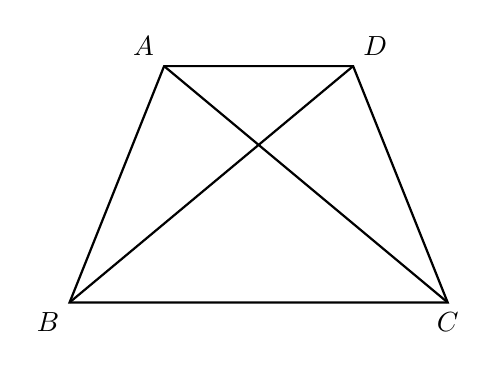
\begin{tikzpicture}[>=stealth, thick, scale=1.2]
    % --- 1. 定义核心点坐标 ---
    % 定义底边顶点 B，以及梯形的高度和宽度参数
    \coordinate (B) at (0,0);
    \coordinate (C) at (4,0);
    \coordinate (A) at (1,2.5);
    \coordinate (D) at (3,2.5);

    % --- 2. 绘制主要几何轮廓 ---
    % 绘制梯形 ABCD
    \draw (A) -- (B) -- (C) -- (D) -- cycle;

    % 绘制对角线 AC 和 BD
    \draw (A) -- (C);
    \draw (B) -- (D);

    % --- 4. 标注顶点文字 ---
    % 使用 anchor 确保文字不遮挡线条
    \node[above left]  at (A) {$A$};
    \node[above right] at (D) {$D$};
    \node[below left]  at (B) {$B$};
    \node[below]       at (C) {$C$};

\end{tikzpicture}

\end{document}